%----------------------------------------------------------------------------------------
  %	PACKAGES AND OTHER DOCUMENT CONFIGURATIONS
  %----------------------------------------------------------------------------------------
  % \RequirePackage{silence}
  % \WarningsOff*
  % \batchmode
  % \documentclass[twoside,twocolumn]{article}
  \documentclass[utf8]{ctexart}
  \raggedbottom
  \usepackage{ctex}
  
  % ======== 通用设置 ========
  
  % 页面布局
  \usepackage{geometry}
  \geometry{a4paper,top=3cm,bottom=3cm,inner=2cm,outer=2cm,marginparwidth=1.8cm}
  
  % 兼容utf8的字体设置
  \setmainfont{CMU Serif}
  % \setCJKmainfont[ItalicFont={华文楷体}]{思源宋体 CN}
  % 思源宋体CN下载:https://github.com/adobe-fonts/source-han-serif/releases/download/2.002R/14_SourceHanSerifCN.zip
  
  % 必备数学套件
  \usepackage{amsmath,amsthm,amsfonts,amssymb}
  \usepackage{bm,bbm,upgreek}
  
  % 图片导入配置
  \usepackage{graphicx}
  \usepackage[export]{adjustbox}
  % 搜寻图片的路径
  \graphicspath{ {./images/} }
  
  % 图注设置
  \usepackage[small,labelfont=bf,up,up,margin=2em]{caption} % Custom captions under/above floats in tables or figures
  
  % 公式、图等的编号设置
  \usepackage{chngcntr}
  %   \counterwithout{figure}{chapter}
  %   \counterwithin{equation}{section}
  
  % 列表设置
  \usepackage{enumitem} % Customized lists
  \setlist[itemize]{itemsep=0pt} % Make itemize lists more compact
  \setlist[enumerate]{itemsep=0pt,parsep=0pt,label={[\arabic*]}}
  
  % 页眉页脚
  \usepackage{fancyhdr}
  \pagestyle{fancy}
  \fancyfoot[EL,OR]{\bfseries· \thepage ·}
  \fancyfoot[C]{}
  \renewcommand{\headrulewidth}{0pt}
  
  % 标题设置
  \usepackage{titling} % Customizing the title section
  % 摘要环境设置(book模板中无效)
  \usepackage{abstract} % Allows abstract customization
  \renewcommand{\abstractnamefont}{\normalfont\bfseries} % Set the "Abstract" text to bold
  \renewcommand{\abstracttextfont}{\normalfont\small\itshape} % Set the abstract itself to small italic text
  
  % 色彩
  \usepackage[svgnames]{xcolor} % added by Wenyin for color
  
  % 超链接设置
  \usepackage[
  colorlinks,
  linkcolor=blue,
  bookmarksnumbered=true,
  bookmarksopen=true
  ]{hyperref}
  % unicode支持:pdf目录可以正确显示公式
  \hypersetup{unicode, psdextra}
  % PDF目录自定义
  \usepackage{bookmark}
  \bookmarksetup{
  	open,
  	numbered,
  	addtohook={%
  		\ifnum\bookmarkget{level}=0 % chapter
  		\bookmarksetup{bold,color=orange}%
  		\fi
  	}
  }
  
  
  
  
  % ======== 可选设置 ========
  
  % for multiple references with dash
  \usepackage[noadjust]{cite}
  \renewcommand{\citedash}{--}    % when \usepackage{cite}
  
  % 额外数学包
  \usepackage{mathrsfs} 	% for \mathscr
  \usepackage{mathtools} 	% for $\intertext{text}$
  \usepackage{breqn}		% 一个可以自动公式断行的公式环境,效果一般
  \usepackage{mhchem} 	%化学式
  \usepackage{esint}
  
  % 表格类
  \usepackage{booktabs} 	% Horizontal rules in tables
  %\usepackage{longtable}	% 长表格
  %\usepackage{tabu}		% 强大的表格包
  %\usepackage{supertabular}
  
  % 杂技
  \usepackage{multirow}	% 多栏布局
  \usepackage{ulem}		% 下划线
  \usepackage{tikz}		% 绘图工具
  \usepackage{framed}		% 文字加框
  \usepackage{setspace}	% 设置行间距等
  \usepackage{minitoc}	% 小目录
  %\usepackage{tcolorbox}	% 多彩盒子工具,巨复杂
  %\tcbuselibrary{skins,breakable,raster}
  \usepackage{float}		% 图片位置:H
  \usepackage{multicol}	% 普通多栏布局
  
  % 多文件
  \usepackage{subfiles}
  
  %代码抄录
  \usepackage{shortvrb}
  	% \MakeShortVerb|*		%|*·|*可以直接原文抄录为texttt
  %\usepackage{listings}
  %\lstset{
  	%	language=[LaTeX]TeX,					%语言
  	%	backgroundcolor=\color{yellow!10},			%背景颜色
  	%	basicstyle=\small\ttfamily,				%基本字格式
  	%	keywordstyle=\bfseries\color{purple},		%关键字格式
  	%	commentstyle=\color{gray},				%注释格式
  	%	numbers=left,						%行号
  	%	numberstyle=\ttfamily\small,				%行号格式
  	%	breaklines,							%允许断行
  	%	frame=shadowbox,						%外框线
  	%	escapeinside={<@}{@>},					%逃逸部分,还给Latex编码
  	%	lineskip=0pt,						%行距
  	%	xleftmargin=0.05\linewidth,
  	%	xrightmargin=0.05\linewidth,				%盒子宽度
  	%	morekeywords={rowfont}					%更多自定义关键词
  	%	}
  
  
  
  % 段落分栏包,实现中英对照排版的核心工具
  \usepackage{paracol}
  \setlength{\columnseprule}{0.5pt}
  \setlength{\columnsep}{2em}
  \columnratio{0.4}
  
  
  % ======== 自定义命令 ========
  
  % 数学自定义
  \newcommand{\vect}[1]{\mathbf{\boldsymbol{#1}}} % works for both English and Greek letters, but it does not work with mathtime pro lite fonts, see https://tex.stackexchange.com/questions/3535/bold-math-automatic-choice-between-mathbf-and-boldsymbol-for-latin-and-greek 
  % \newcommand{\matr}[1]{\boldsymbol{\mathrm{#1}}} % \matrix is defined in LaTeX2e kernel
  \newcommand{\tens}[1]{\boldsymbol{\mathrm{#1}}}
  \newcommand\ii{\symup{i}}
  \newcommand\ee{\symup{e}}
  \newcommand\dd{\symup{d}}
  \newcommand\ppi{\symup{\pi}}	%常用的正体字符:i,e,d,\pi
  
  \renewcommand{\paragraph}[1]{\textbf{#1}}
  % ====== 对照排版的设置 ======
  
  % ===中英文对照排版,四六开===
  \columnratio{0.4}
  \newcommand\mainskip{-5pt}
  \newcommand\enzhbox[2]{
  	\quad\par \begin{paracol}{2} \colseprulecolor{black} 
  		\begin{spacing}{1.0}
  			\footnotesize  #1
  		\end{spacing}
  		\switchcolumn[1] 
  		#2
  	\end{paracol} \quad\par
  }
  
  % ===中英文对照排版,五五开===
  %\columnratio{0.48}
  %\newcommand\mainskip{-5pt}
  %\newcommand\enzhbox[2]{
  %	\quad\par \begin{paracol}{2} \colseprulecolor{black} 
  %		\begin{spacing}{1.0}
  %			\small  #1
  %		\end{spacing}
  %		\switchcolumn[1] 
  %		#2
  %	\end{paracol} \quad\par
  %}
  
  % === 仅英文(#1)/仅中文(#2) ===
  % \newcommand\mainskip{5pt}
  % \newcommand\enzhbox[2]{#1}
  %\newcommand\enzhbox[2]{#2}
  
  %%编号层级表
  %%-1 part
  %%0 chapter
  %%1 section
  %%2 subsection
  %%3 subsubsection
  %%4 paragraph
  %%5 subparagraph
  % % 章节标题编号深度
  % \setcounter{secnumdepth}{3}		
  % % 目录深度
  % \setcounter{tocdepth}{2}
  % % 小目录深度
  % \setcounter{minitocdepth}{3}
  % \renewcommand\mtctitle{本章目录}
  
  %----------------------------------------------------------------------------------------
  %	TITLE SECTION
  %----------------------------------------------------------------------------------------
  
  % \setlength{\droptitle}{-4\baselineskip} % Move the title up
  
  % \pretitle{\begin{center}\Huge\bfseries} % Article title formatting
  % 	\posttitle{\end{center}} % Article title closing formatting
 \title{压力和电感对异型托卡马克垂直稳定性的影响\\ \Large{PRESSURE AND INDUCTANCE EFFECTS ON THE VERTICAL STABILITY OF SHAPED TOKAMAKS }}  \author{D.J. WARD,  A. BONDESON,  F. HOFMANN et al.}
  
  \newcommand\paperref{D.J. WARD. 1993 Nucl. Fusion 33 821}
   
  \date{\paperref}
  \fancyhead[C]{\small \paperref}
  \fancyhead[L,R]{}
  \renewcommand\headrulewidth{0.6pt}
  \renewcommand{\maketitlehookd}{%
  	\begin{abstract}
 {数值计算显示了压力和电感对异型托卡马克垂直稳定性的影响。高$\epsilon \beta_{p}$ 值可提高 "笛 "形托卡马克的垂直稳定性,但对反 "笛 "形托卡马克来说则会失稳。对于细长横截面,压力效应可以很好地描述为稳定内电感$l_{\mathrm{i}}$ 的最大值与$\epsilon \beta_{\mathrm{p}}$的线性关系,其系数取决于几何形状,并随三角形变而增加。对于 TCV 型和 DIII-D 型横截面,$l_{\mathrm{i}}$  与 $\epsilon \beta_{\mathrm{p}}$ 的关系显示了稳定图。电流剖面效应主要取决于壁的位形:如果壁很近,$l_{\mathrm{j}}$  的低值具有稳定作用,但如果没有壁,则会增加不稳定性的驱动力。这两种效应之间的竞争是针对具有离散外部导体的位形而考虑的。
}\\ \indent  Numerical calculations are presented to show the influence of pressure and inductance on the vertical stability of shaped tokamaks. High values of $\epsilon \beta_{p}$ improve the vertical stability of dee shaped tokamaks but are destabilizing for an inverse dee. For elongated cross-sections, the pressure effect is well described by a linear dependence of the maximum value of the stable internal inductance $l_{\mathrm{i}}$ on $\epsilon \beta_{\mathrm{p}}$, with a coefficient that depends on the geometry and increases with the triangularity. Stability diagrams are shown in terms of $l_{\mathrm{i}}$ versus $\epsilon \beta_{\mathrm{p}}$ for TCV- and DIII-D-like crosssections. Current profile effects depend critically on the wall configuration: low values of $l_{\mathrm{j}}$ are stabilizing if the wall is close, but increase the driving force of the instability in the absence of a wall. The competition between these two effects is considered for a configuration with discrete external conductors.
  	\end{abstract}
  }
  
  %----------------------------------------------------------------------------------------
  
  \begin{document}
  \begin{sloppypar}
  	% \nonstopmode 
  	% \WarningsOff[latex] 
  % 公式环境的一些设置
  \allowdisplaybreaks[3]  
  \setlength{\abovedisplayskip}{-6pt}
  \setlength{\belowdisplayskip}{10pt}
  \setlength{\abovedisplayshortskip}{0pt}
  \setlength{\belowdisplayshortskip}{0pt}
  \setlength{\parskip}{\mainskip}
  
  	% \setcounter{chapter}{3}
  	\maketitle
  
  % ==document boby begins
  
  
 \section{引言}
 {  \small INTRODUCTION \par }
 
\enzhbox{  Modern tokamaks are generally designed so as to take advantage of the increased current capability of an elongated cross-section and the resulting improvement of the beta limit \textcolor{green!50!black}{[1,2]} and confinement time \textcolor{green!50!black}{[3]}. A well known drawback of elongation is vertical instability $\textcolor{green!50!black}{[4,5]}$, which requires the use of conducting walls close to the plasma assisted by active feedback stabilization on the $L / R$ time-scale of the resistive wall. Work on the DIII-D tokamak has established that vertical instability is the factor that limits the achievable elongation \textcolor{green!50!black}{[2, 6]}. For the TCV experiment \textcolor{green!50!black}{[7]} in Lausanne, designed for a maximum elongation of $\kappa=3$, the vertical stability is a major issue, and we have therefore investigated numerically the operational limits due to the vertical instability and how these depend on, e.g., the shape of the plasma cross-section and the equilibrium profiles.}{
现代托卡马克的设计通常是为了利用拉长横截面带来的更大电流能力,以及由此带来的贝塔极限\textcolor{green!50!black}{[1,2]}和约束时间\textcolor{green!50!black}{[3]}的改善。拉长横截面的一个众所周知的缺点是垂直不稳定性$\textcolor{green!50!black}{[4,5]}$,这就要求使用靠近等离子体的导电壁,并在电阻壁的$L / R$ 时间尺度上辅助以主动反馈稳定。在 DIII-D 托卡马克上进行的工作已经确定,垂直不稳定性是限制可实现的伸长率的因素\textcolor{green!50!black}{[2, 6]}。洛桑 TCV 实验\textcolor{green!50!black}{[7]}的设计最大伸长率为 $\kappa=3$,垂直不稳定性是一个主要问题,因此我们用数值方法研究了垂直不稳定性导致的运行极限,以及这些极限与等离子体截面形状和平衡剖面等因素的关系。}
  
 
\enzhbox{  It is found experimentally \textcolor{green!50!black}{[8]} that the vertical stability of strongly elongated tokamaks is favoured by a low internal inductance $l_{\mathrm{i}}$, because this increases the coupling of the plasma current to the surrounding wall. Vertical stability requires an internal inductance less than some threshold value $l_{\mathrm{i}, \text { crit }}$, which decreases with increasing elongation and wall distance. Here, we mean by $l_{\mathrm{i}, \text { crit }}$ the value of $l_{\mathrm{i}}$ for which a plasma surrounded by a realistic resistive wall has an $n=0$ growth rate, $\gamma_{\text {crit }}$, below which the vertical position can be controlled by a practical feedback system.}{
实验\textcolor{green!50!black}{[8]}发现,低内电感$l_{\mathrm{i}}$有利于强拉伸托卡马克的垂直稳定性,因为这会增加等离子体电流与周围壁面的耦合。垂直稳定性要求内电感小于某个阈值$l_{\mathrm{i}, \text { crit }}$,而这个阈值会随着伸长率和壁间距的增加而减小。这里,我们所说的 $l_{\mathrm{i}, \text { crit }}$ 是指 $l_{\mathrm{i}}$ 的值,在该值下,被实际电阻壁包围的等离子体的增长率为 $n=0$  ,即 $\gamma_{\text {crit }}$ ,低于该值,垂直位置可由实际反馈系统控制。}
  
  
 
\enzhbox{  Our principal result is that $l_{\mathrm{i}, \text { crit }}$ is strongly influenced by pressure in combination with triangular shaping of the cross-section. We find numerically that $l_{i, \text { crit }}$ is an approximately linear function of $\epsilon \beta_{\mathrm{p}}$, independent of the details of the current profile and aspect ratio, but sensitively dependent on the geometry of the crosssection and the distance to the wall. For the usual dee shape, pressure is stabilizing, i.e. $l_{\mathrm{i} \text {, crit }}$ increases with $\epsilon \beta_{\mathrm{p}}$, whereas in an inverse dee, pressure is destabilizing. The increased upper limit in internal inductance for a normal dee is a favourable effect, not only because it makes it possible to reach a higher elongation, but also because the beta limit $\textcolor{green!50!black}{[2,9]}$ and confinement time \textcolor{green!50!black}{[10]} improve with the internal inductance at fixed elongation. Reference \textcolor{green!50!black}{[2]} shows convincing evidence that the optimum condition for reaching high beta is at the intersection of the $n=0$ and $n=1$ stability boundaries, where $n$ is the toroidal mode number.}{
我们的主要结果是,$l_{\mathrm{i}, \text { crit }}$  受到压力和横截面三角形变的强烈影响。我们通过数值计算发现,$l_{i, \text { crit }}$ 与$\epsilon \beta_{\mathrm{p}}$近似为线性函数,与电流剖面的细节和环径比无关,但与横截面的几何形状和到壁的距离有关。对于通常的笛形,压力是稳定的,即 $l_{\mathrm{i} \text {, crit }}$  随 $\epsilon \beta_{\mathrm{p}}$ 的增加而增加,而在反笛形中,压力是失稳的。正常氐形的内电感上限增加是一个有利的影响,这不仅是因为它可以达到更高的伸长率,还因为在伸长率固定的情况下,贝塔极限$\textcolor{green!50!black}{[2,9]}$ 和约束时间\textcolor{green!50!black}{[10]}会随着内电感的增加而提高。参考文献\textcolor{green!50!black}{[2]}提供了令人信服的证据,证明达到高贝塔值的最佳条件是$n=0$ 和$n=1$ 稳定边界的交叉点,其中$n$ 是环模数。}
  
 
\enzhbox{  The stabilizing effect of low inductance $l_{\mathrm{i}}$ is due to improved wall coupling in configurations with a completely surrounding wall. However, broad current profiles tend to give higher ideal growth rates with the wall at infinity. Here, we shall discuss the competition of these effects for a configuration where the wall is replaced by discrete conductors.}{
低电感$l_{\mathrm{i}}$ 的稳定效应是由于在完全环绕壁的位形中,壁耦合得到了改善。然而,宽电流剖面往往会使壁面处于无穷远处的理想增长率更高。在此,我们将讨论在壁被离散导体取代的位形下,这些效应的竞争情况。}
  
 \section{TCV 和 DII-D 截面的稳定图}
 {  \small STABILITY DIAGRAMS FOR TCV AND DIII-D CROSS-SECTIONS \par }
 
\enzhbox{  Figure 1 shows the limit in internal inductance $l_{\mathrm{i}, \text {, rit }}$ as a function of $\epsilon \beta_{p}$ for three different classes of current profiles in a 'TCV cross-section' at aspect ratio $A=1 / \epsilon=R_{0} / a=3.7$ (curves $1-3$ ). The following definitions are used for the poloidal beta:\\}{
\textcolor{blue}{图 1} 显示了在环径比为 $A=1 / \epsilon=R_{0} / a=3.7$  的 「TCV 截面 」中,三类不同电流剖面的内电感 $l_{\mathrm{i}, \text {, rit }}$  极限与 $\epsilon \beta_{p}$  的函数关系(曲线 $1-3$  )。以下定义用于极向贝塔:( )。}
 \begin{align*}
 	 \beta_{\mathrm{p}} \equiv \frac{4}{\mu_{0} I_{\mathrm{p}}^{2} R_{0}} \int_{\mathrm{pt}} p \mathrm{~d}^{3} x
 \end{align*}
  
 
\enzhbox{  \noindent and internal inductance\\}{
\noindent 和内部电感}
  \begin{align*}
  l_{\mathrm{i}} \equiv \frac{2}{\mu_{0}^{2} I_{\mathrm{p}}^{2} R_{0}} \int_{\mathrm{p} \ell} B_{\mathrm{p}}^{2} \mathrm{~d}^{3} x
  \end{align*}
  
 
\enzhbox{  The plasma-vacuum boundary is specified as\\}{
等离子体-真空边界被指定为}
  \begin{gather*}
  	R / a=A+\cos (\theta+\delta \sin \theta+\lambda \sin 2 \theta) \tag{1}\\
  Z / a=\kappa \sin \theta 
  \end{gather*}
  
  
 
  
 
\enzhbox{  \noindent and the geometry referred to as 'TCV dee' has elongation $\kappa=3$, triangularity $\delta=0.5$ and squareness $\lambda=0.2$. Equilibria have been computed with the CHEASE code \textcolor{green!50!black}{[11]} and stability with the NOVA-W code \textcolor{green!50!black}{[12]}, which is capable of computing the growth rates of $n=0$ modes with a resistive wall, as well as with an ideal wall or with no wall. Figure 1 refers to resistive wall instabilities (cases that are stable with an ideal wall), and it is assumed that the mode can be stabilized by active feedback control if the resistive wall growth time is longer than $7 \%$ of the $L / R$ time of the wall (more precisely, for its ' $m=1$ ' eigenmode), i.e. 0.5 ms . The conducting wall represents the TCV vacuum vessel \textcolor{green!50!black}{[7]}.}{
\noindent 而被称为 「TCV dee 」的几何形状具有伸长率$\kappa=3$、三角形变$\delta=0.5$ 和方形$\lambda=0.2$。利用 CHEASE 代码\textcolor{green!50!black}{[11]}计算了平衡,利用 NOVA-W 代码\textcolor{green!50!black}{[12]}计算了稳定性,该代码能够计算电阻壁模、理想壁模或无壁模的$n=0$ 增长率。\textcolor{blue}{图 1} 指的是电阻壁不稳定性(使用理想壁时稳定的情况),假设如果电阻壁增长时间长于电阻壁$L / R$ 时间的$7 \%$ (更准确地说,是其'$m=1$ '本征模),即 0.5 毫秒,则可以通过主动反馈控制来稳定该模式。导电壁代表 TCV 真空腔体 \textcolor{green!50!black}{[7]}。}
  \begin{figure}[H]
  	\centering
  	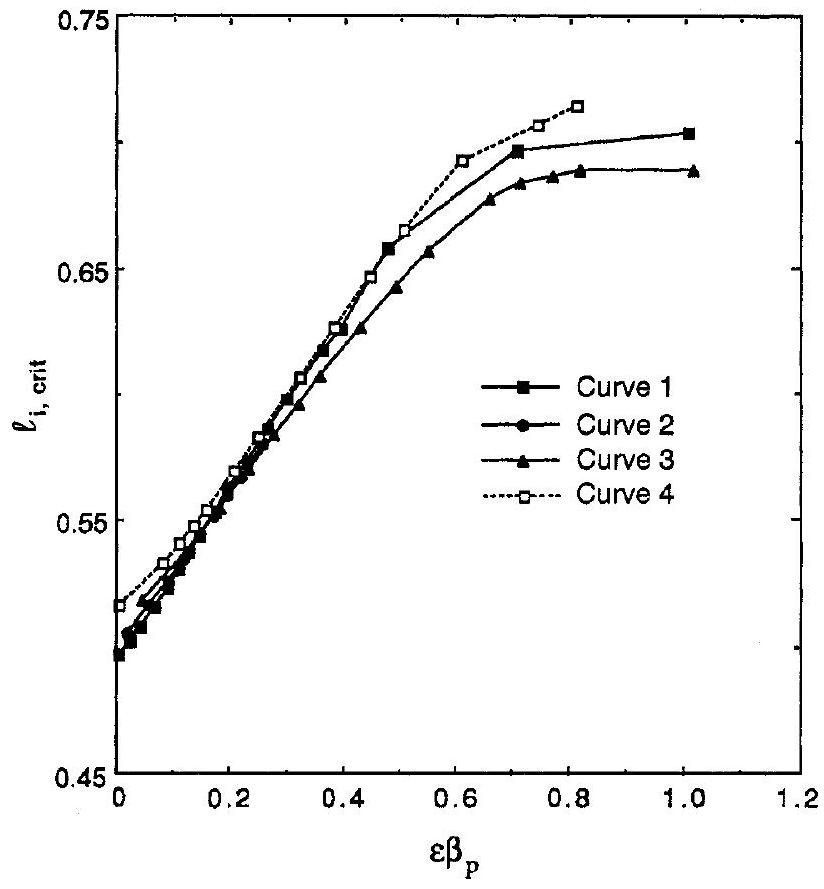
\includegraphics[max width=0.85\textwidth,max height=0.3\textheight]{2025_01_10_a0135324997886412d98g-3}
 \caption{\uline{Vertical stability diagram in terms of $1_{i, \text { crit }}$ and $\epsilon \beta_{p}$ for the TCV configuration. Curves $1-3$ show the results for the standard TCV configuration for three different types of current profiles. Curve 4 shows the results for the TCV plasma and wall shape expanded to an aspect ratio of $\mathrm{R}_{0} / \mathrm{a}=7.0$ for the first current profile.\\}\\以 $1_{i, \text { crit }}$  和 $\epsilon \beta_{p}$  表示的 TCV 位形的垂直稳定性图。曲线 $1-3$  显示了标准 TCV 位形在三种不同类型电流剖面下的结果。曲线 4 显示了 TCV 等离子体和壁形扩展到第一种电流剖面的环径比 $\mathrm{R}_{0} / \mathrm{a}=7.0$  时的结果。}
  	\label{fig1.}
  \end{figure}
  
   % ==AUTO MOVED 
  
 
\enzhbox{  Several conclusions can be drawn from Fig. 1. Firstly, the limit in $l_{\mathrm{i}}$ is the same function of $\beta_{\mathrm{p}}$ for the three different classes of current profiles. The three current profiles differ significantly, and Fig. 2 shows the profiles 1 and 3 for the surface averaged toroidal current density $I^{*}$ at the point $l_{\mathrm{i}}=l_{\mathrm{i}, \text { crit }}$ at low and high pressures ( $\epsilon \beta_{\mathrm{p}}=0$ and 0.5 , respectively). (The pressure profiles have been chosen as uniformly scaled versions of those that give the ballooning limit with a given $I^{*}$ profile.) Secondly, curve 4 refers to an equilibrium with a larger aspect ratio, $A=7$. The large aspect ratio result coincides almost exactly with that for $A=3.7$ when it is plotted in terms of $l_{\mathrm{i}}$ and $\epsilon \beta_{\mathrm{p}}$. Thus, for a fixed, elongated cross-section (but with varying current profile and aspect ratio) $n=0$ stability requires $l_{\mathrm{i}}<l_{\mathrm{i}, \text { crit }}\left(\epsilon \beta_{\mathrm{p}}\right.$ ), and for $\epsilon \beta_{\mathrm{p}}$ not too large $l_{\mathrm{i}, \text { crit }}$ is almost linear in $\epsilon \beta_{\mathrm{p}} ; l_{\mathrm{i}, \text { crit }} \approx l_{\mathrm{i}, 0}+c \epsilon \beta_{\mathrm{p}}$.}{
从\textcolor{blue}{图 1} 中可以得出几个结论。首先,对于三类不同的电流剖面,$l_{\mathrm{i}}$  中的极限是$\beta_{\mathrm{p}}$  的相同函数。这三种电流剖面差别很大,\textcolor{blue}{图 2} 显示了在低压和高压(分别为 $\epsilon \beta_{\mathrm{p}}=0$  和 0.5 ,)下,$l_{\mathrm{i}}=l_{\mathrm{i}, \text { crit }}$  点的表面平均环形电流密度 $I^{*}$  的剖面 1 和 3。(压力剖面是根据给定的$I^{*}$ 剖面给出气球极限的压力剖面的均匀缩放版本选择的)。其次,曲线 4 指的是具有较大环径比 $A=7$ 的平衡。如果用 $l_{\mathrm{i}}$  和 $\epsilon \beta_{\mathrm{p}}$ 来表示,大环径比的结果与 $A=3.7$  的结果几乎完全吻合。因此,对于固定的细长截面(但电流剖面和环径比不同),$n=0$  稳定性要求 $l_{\mathrm{i}}<l_{\mathrm{i}, \text { crit }}\left(\epsilon \beta_{\mathrm{p}}\right.$  ),而对于 $\epsilon \beta_{\mathrm{p}}$ 不是太大的 $l_{\mathrm{i}, \text { crit }}$  几乎与 $\epsilon \beta_{\mathrm{p}} ; l_{\mathrm{i}, \text { crit }} \approx l_{\mathrm{i}, 0}+c \epsilon \beta_{\mathrm{p}}$ 成线性关系。}
  
  
 
\enzhbox{  Figure 3 shows the corresponding result for a DIII-D-like cross-section, $\kappa=2.5, \delta=0.6, \lambda=0$ and $A=3$. Here, the resistive wall was chosen to be conformal to the plasma boundary, and two different minor radii have been considered for the wall; $d=1.3 a$ and $d=1.4 a$. The result is similar to that for the TCV dee shape in that the critical internal inductance increases with $\epsilon \beta_{p}$; however, the dependence is much stronger for the DIII-D cross-section. For the DIII-D-like case with $d=1.3 a$, we have $l_{\mathrm{i}, \text { crit }} \approx l_{\mathrm{i}, 0}+c \in \beta_{\mathrm{p}}$, with $c \approx 1.8$, which is much larger than for the TCV dee, where $c \approx 0.34$.}{
\textcolor{blue}{图 3} 显示了类似 DIII-D 的横截面 $\kappa=2.5, \delta=0.6, \lambda=0$  和 $A=3$ 的相应结果。在这里,电阻壁被选择为与等离子体边界共形,并考虑了两种不同的小半径;$d=1.3 a$  和 $d=1.4 a$ 。结果与 TCV dee 形状类似,临界内电感随 $\epsilon \beta_{p}$ 的增加而增加;但对于 DIII-D 截面,这种依赖性要强得多。对于具有 $d=1.3 a$ 的 DIII-D 类情况,我们有 $l_{\mathrm{i}, \text { crit }} \approx l_{\mathrm{i}, 0}+c \in \beta_{\mathrm{p}}$ ,具有 $c \approx 1.8$ ,这比 TCV dee 的 $c \approx 0.34$ 大得多。}
  
 
\enzhbox{  Also shown in Fig. 3 are two additional cases that compare the variation of the shape at the two different elongations. The first case has the high elongation ( $\kappa=3$ ) of the TCV dee shape, but with higher triangularity ( $\delta=0.6$ ) and no squareness $(\lambda=0)$. Because of the poor coupling of equilibria with this shape to the TCV vacuum vessel, we use a conformal wall with the distance chosen ( $d=1.275 a$ ) to give the same value of $l_{i, 0}$ as the TCV dee configuration at zero pressure. The stability boundary for this case has a slope almost as large as that for the DIII-D-like crosssection. The other case has the same elongation ( $\kappa=2.5$ ) as the DIII-D-like cross-section, but has the triangularity and squareness parameters corresponding to the TCV dee shape ( $\delta=0.5$ and $\lambda=0.2$ ). This case gives a line with an intermediate slope $c$ which is closer to that of the TCV dee shape. Thus, triangularity increases the slope and elongation decreases it, and in comparing the DIII-D and TCV dee shapes the effect of triangularity is dominant.}{
\textcolor{blue}{图 3} 还显示了另外两种情况,比较了两种不同伸长率下的形状变化。第一种情况具有 TCV dee 形状的高伸长率($\kappa=3$ ),但具有较高的三角形变($\delta=0.6$ ),没有方形$(\lambda=0)$。由于这种形状的平衡与 TCV 真空腔体的耦合性较差,我们使用保形壁,其距离选择 ( $d=1.275 a$  ) 使 $l_{i, 0}$  值与零压下的 TCV dee 位形相同。这种情况下的稳定边界斜率几乎与类似 DIII-D 断面的稳定边界斜率一样大。另一种情况的伸长率($\kappa=2.5$  )与类 DIII-D 断面相同,但具有与 TCV dee 形状相对应的三角形变和方形参数($\delta=0.5$  和 $\lambda=0.2$  )。这种情况下的直线具有中间斜率$c$ ,更接近 TCV dee 形状的斜率。因此,三角形变会增加斜率,而伸长会减小斜率,在比较 DIII-D 和 TCV dee 形状时,三角形变的影响占主导地位。}
  
 
\enzhbox{  The stability threshold, of course, depends on the assumptions concerning the critical growth rate $\gamma_{\text {crit }}$. If the critical growth rate is changed, the main effect is a uniform shift of $l_{\mathrm{i}, \text { crit }}\left(\epsilon \beta_{\mathrm{p}}\right)$, with only a small effect on the slope $c$. For example, if $\gamma_{\text {crit }}$ for the TCV case, Fig. 1, is increased by $50 \%$ (this relaxes the demands on the feedback system), then the value of $l_{\mathrm{i}, 0}$ increases from 0.494 to 0.519 , while the slope $c$ increases by about $8 \%$. For the DIII-D-like case, if $\gamma_{\text {crit }}$ is increased by $50 \%$ the value of $l_{\mathrm{i}, 0}$ increases considerably, from 0.521 to 0.667 , but the value of the slope $c$ increases by only $3 \%$.\\ Note that Fig. 3 does not apply literally to DIII-D conditions, e.g. with respect to the assumed value of $\gamma_{\text {crit }} \tau_{\text {wall }}$. Furthermore, our definitions of $\beta_{\mathrm{p}}$ and $l_{\mathrm{i}}$ differ from those used in, for example, Ref. \textcolor{green!50!black}{[2]} by a shape dependent factor. For the DIII-D shape our values are smaller by a factor of approximately 1.5 . Improved vertical stability at high $\beta$ has been observed in DIII-D and was attributed to the broader current profiles at high $\beta$ due to a large fraction of bootstrap current \textcolor{green!50!black}{[2]}. Our calculations show that finite $\beta$ also has a direct effect on vertical stability, and this effect is significant for the DIII-D cross-section.}{
当然,稳定性阈值取决于临界增长率 $\gamma_{\text {crit }}$ 的假设。如果临界增长率发生变化,主要影响是$l_{\mathrm{i}, \text { crit }}\left(\epsilon \beta_{\mathrm{p}}\right)$的均匀移动,对斜率$c$的影响很小。例如,如果\textcolor{blue}{图 1} 中 TCV 情况下的 $\gamma_{\text {crit }}$ 增加 $50 \%$ (这弛豫了对反馈系统的要求),则 $l_{\mathrm{i}, 0}$  值从 0.494 增加到 0.519,而斜率 $c$ 增加约 $8 \%$ 。对于类似 DIII-D 的情况,如果$\gamma_{\text {crit }}$增加$50 \%$ ,$l_{\mathrm{i}, 0}$ 的值会大幅增加,从 0.521 增加到 0.667,但斜率$c$的值仅增加$3 \%$。此外,我们对 $\beta_{\mathrm{p}}$  和 $l_{\mathrm{i}}$  的定义与参考文献\textcolor{green!50!black}{[2]}等所使用的定义不同。\textcolor{green!50!black}{[2]}中的定义有一个因形状而异的系数。对于 DIII-D 形状,我们的数值要小大约 1.5 倍。在DIII-D中观察到高$\beta$ 处的垂直稳定性有所提高,这归因于高$\beta$ 处的电流剖面更宽,这是因为自举电流的比例很大\textcolor{green!50!black}{[2]}。我们的计算表明,有限 $\beta$  也对垂直稳定性有直接影响,而且对 DIII-D 截面的影响很大。}
  \begin{figure}[H]
  	\centering
  	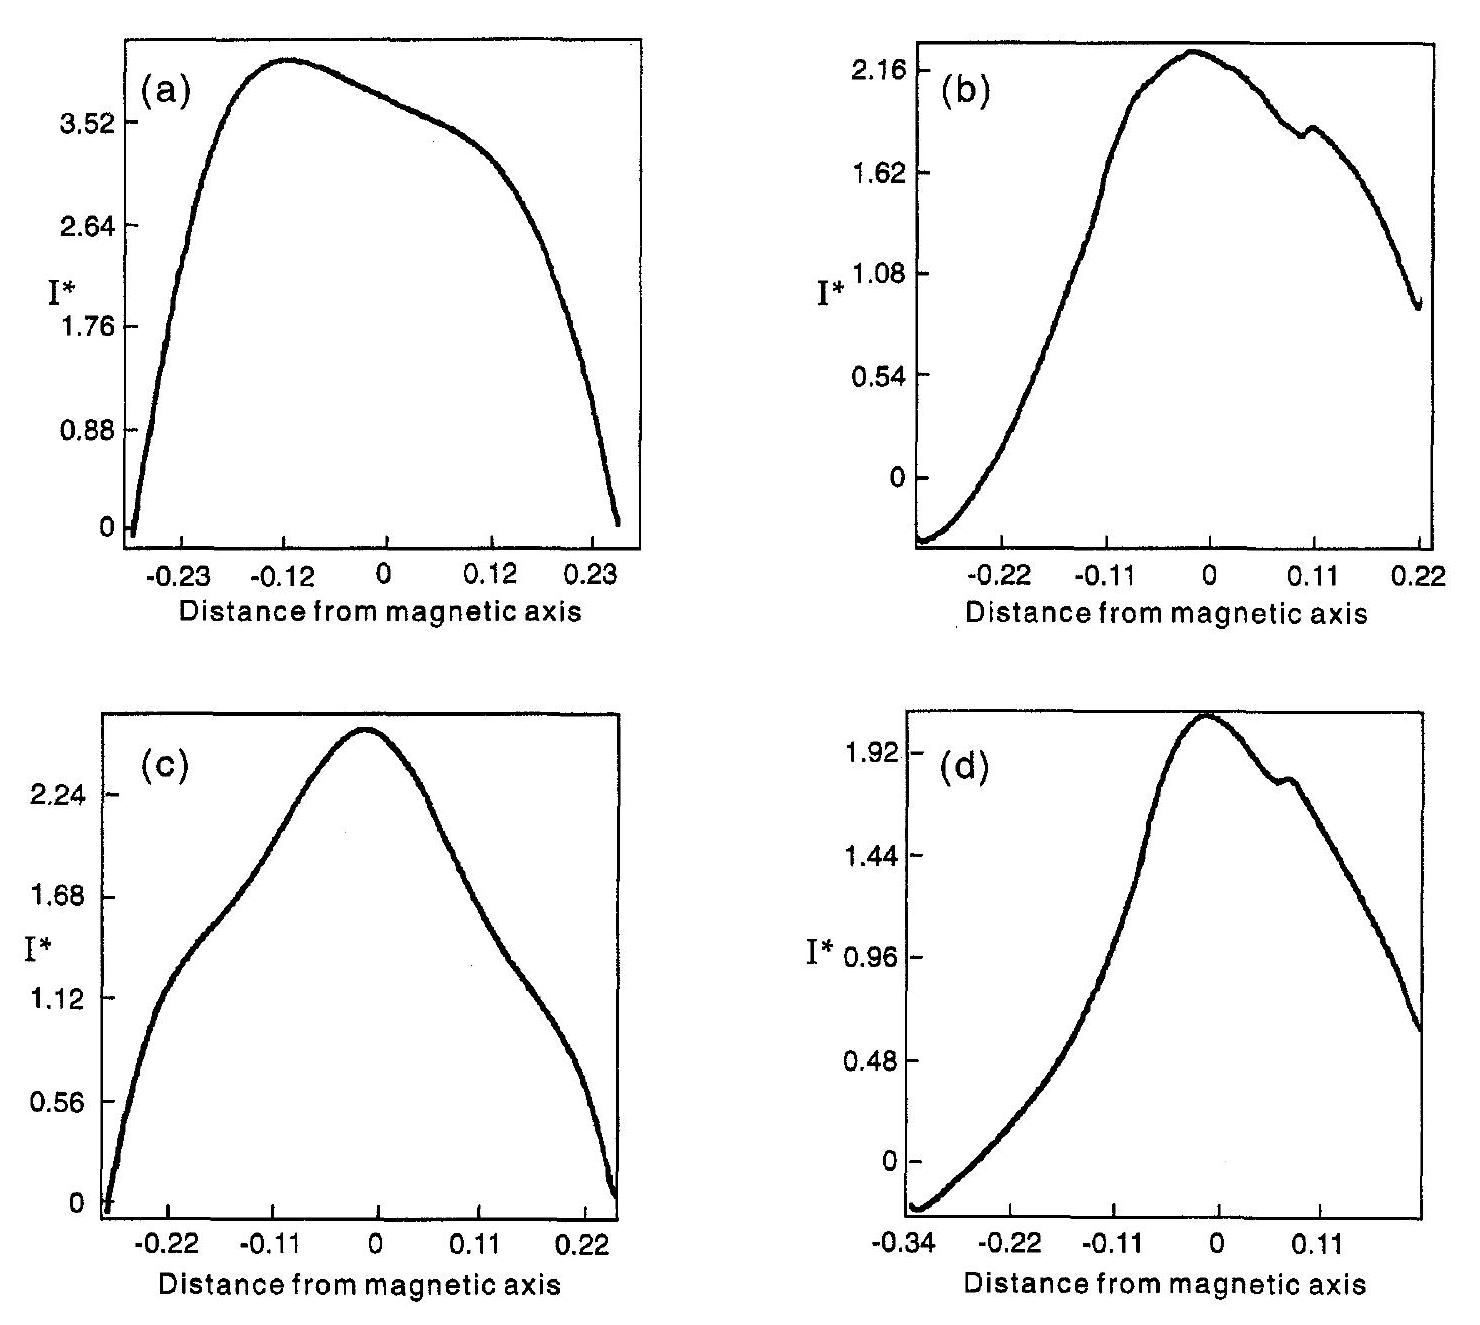
\includegraphics[max width=0.85\textwidth,max height=0.35\textheight]{2025_01_10_a0135324997886412d98g-4}
 \caption{\uline{Current profiles ( 1 * is the surface averaged toroidal current density) corresponding to curves 1 and 3 of Fig. 1. Both profile types are shown at low and high beta: (a) curve $1, \beta_{p}=0.06$; (b) curve $1, \beta_{p}=0.6$; (c) curve 3, $\beta_{p}=0.06$; (d) curve 3, $\beta_{p}=0.6$.}\\与\textcolor{blue}{图 1} 曲线 1 和 3 相对应的电流剖面(1 * 为表面平均环形电流密度)。两种剖面都显示了低贝塔和高贝塔时的情况:(a)曲线 $1, \beta_{p}=0.06$ ;(b)曲线 $1, \beta_{p}=0.6$ ;(c)曲线 3,$\beta_{p}=0.06$ ;(d)曲线 3,$\beta_{p}=0.6$ 。}
  	\label{fig2.}
  \end{figure}
  
   
  % ==AUTO MOVED 
  
 \section{理论成果简要回顾}
 {  \small BRIEF REVIEW OF THEORETICAL RESULTS \par }
 
\enzhbox{  Several results relevant to the diagrams in Figs 1 and 3 have been obtained previously by analytical [ $4,5,13-15]$, semi-analytical \textcolor{green!50!black}{[16, 17]} or numerical \textcolor{green!50!black}{[18-20]} methods. Quite surprisingly, most of the work on shape, pressure and inductance effects on vertical stability dates from the 1970 s, despite the subsequent development of powerful numerical codes and the fact that experiments are now in regimes where such effects are of importance.\\ Zakharov \textcolor{green!50!black}{[4]} showed that vertical elongation, $\kappa>1$, destabilizes vertical shifts but that a weakly elongated equilibrium can be stabilized by finite aspect ratio effects without the use of a conducting shell. Vertical displacements are stable if the decay index $n$ of the external vertical field satisfies $n \equiv-\left(R_{0} / B_{z}^{\text {ext }}\right)\left(\partial B_{z}^{\text {ext }} / \partial R\right)_{R=R_{0}}>0$.}{
与\textcolor{blue}{图 1} 和\textcolor{blue}{图 3} 中图表相关的一些结果是以前通过分析[$4,5,13-15]$、半分析\textcolor{green!50!black}{[16, 17]}或数值\textcolor{green!50!black}{[18-20]}方法获得的。扎哈罗夫\textcolor{green!50!black}{[4]}指出,垂直伸长$\kappa>1$会使垂直位移失稳,但弱伸长平衡可以通过有限导电率效应来稳定,而无需使用导电壳。如果外部垂直场的衰减指数 $n$  满足 $n \equiv-\left(R_{0} / B_{z}^{\text {ext }}\right)\left(\partial B_{z}^{\text {ext }} / \partial R\right)_{R=R_{0}}>0$ ,则垂直位移是稳定的。}
  \begin{figure}[H]
  	\centering
  	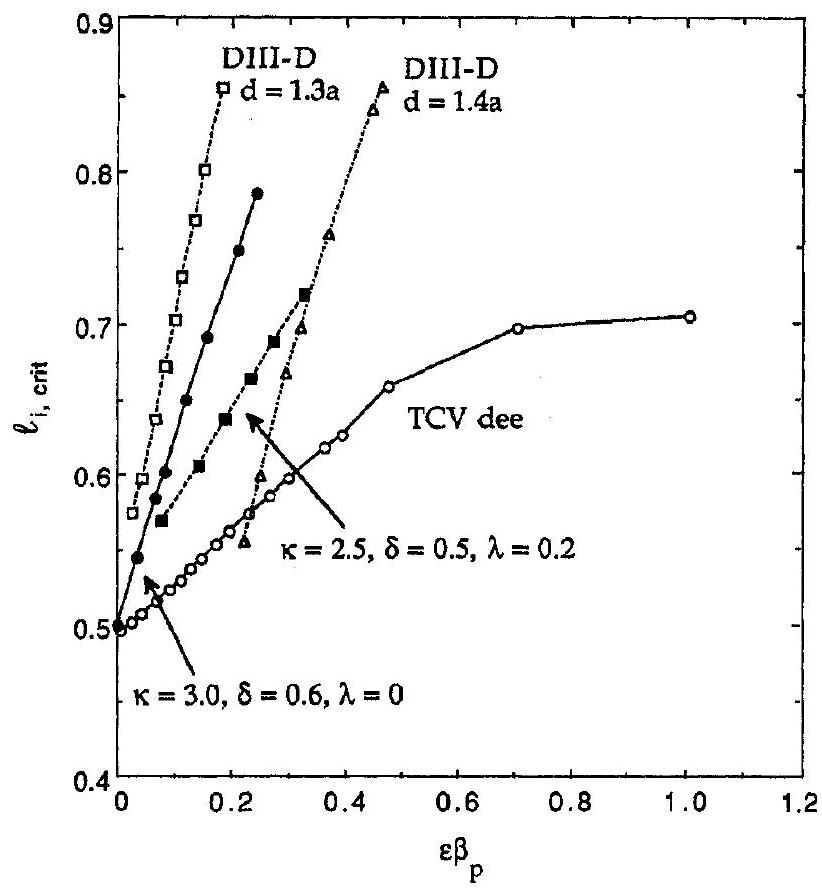
\includegraphics[max width=0.85\textwidth,max height=0.3\textheight]{2025_01_10_a0135324997886412d98g-5}
 \caption{\uline{Vertical stability diagram in terms of $1_{i, \text { crit }}$ and $\epsilon \beta_{p}$ for several equilibria of varying shapes. Two curves are shown for the DIII-D-like equilibrium with two different wall positions. The walls are conformal to the plasma shape at midplane distances of $\mathrm{d}=1.3 \mathrm{a}$ and $\mathrm{d}=1.4 \mathrm{a}$. For comparison, curve 1 from Fig. 1 for the TCV dee configuration is also shown. Two other stability boundaries intermediate between the DIII-D-like and the TCV dee equilibria are shown, with $\kappa=3.0, \delta=0.6, \lambda=0$ and with $\kappa=2.5, \delta=0.5, \lambda=0.2$.}\\几种不同形状平衡的 $1_{i, \text { crit }}$  和 $\epsilon \beta_{p}$  垂直稳定性图。两条曲线显示的是具有两种不同壁面位置的 DIII-D 类平衡。在中面距离为 $\mathrm{d}=1.3 \mathrm{a}$  和 $\mathrm{d}=1.4 \mathrm{a}$ 时,壁与等离子体形状一致。为便于比较,还显示了\textcolor{blue}{图 1} 中 TCV dee 位形的曲线 1。图中还显示了介于类 DIII-D 平衡和 TCV dee 平衡之间的另外两个稳定边界,分别为 $\kappa=3.0, \delta=0.6, \lambda=0$  和 $\kappa=2.5, \delta=0.5, \lambda=0.2$ 。}
  	\label{fig3.}
  \end{figure}
  
   
  % ==AUTO MOVED 
  
 
\enzhbox{  Zakharov's expression \textcolor{green!50!black}{[4,5]} for $n$ implies that a plasma with a flat current profile is vertically stable when\\}{
扎哈罗夫对 $n$  的表达式\textcolor{green!50!black}{[4,5]}意味着,等离子体在电流剖面平坦时是垂直稳定的。}
 \begin{align*}
 	 \kappa-1<\left(\frac{a}{R_{0}}\right)^{2}\left(\frac{3}{4} \ln \frac{8 R_{0}}{a}-\frac{17}{16}\right) \tag{2}
 \end{align*}
 
\enzhbox{  Laval et al. \textcolor{green!50!black}{[13]} showed that an elongated plasma can be stabilized by a conducting wall. For a flat current profile, their stability condition (in the near circular approximation) is\\}{
Laval 等人 \textcolor{green!50!black}{[13]} 的研究表明,拉长的等离子体可以通过导电壁来稳定。对于平坦的电流剖面,他们的稳定条件(近似圆形)为}
  
 \begin{align*}
 	 \kappa-1<2\left(\frac{a}{d}\right)^{2} \tag{3}
 \end{align*}
  
 
\enzhbox{  \noindent where $d$ is the wall radius. Comparison of the conditions (2) and (3) shows that for the elongations, aspect ratios and wall distances typical of modern tokamaks, wall stabilization is far more important than finite aspect ratio effects \textcolor{green!50!black}{[21]}, and the discharges would be strongly unstable without a wall.}{
\noindent 其中 $d$  为壁面半径。条件(2)和(3)的比较表明,对于现代托卡马克典型的伸长率、环径比和壁距,壁稳定远比有限环径比效应更重要\textcolor{green!50!black}{[21]},如果没有壁,放电将强烈不稳定。}
  
  
 
\enzhbox{  The effects of more complex shaping, including finite aspect ratio and pressure effects, were investigated semi-analytically for a surface current distribution by Rebhan and Salat \textcolor{green!50!black}{[17]}. For vertically elongated equilibria, they found that an inverse dee ( $\delta<0$ ) is destabilized by pressure, but a standard dee ( $\delta>0$ ) can be stabilized by pressure (see Fig. 4(a) of Ref. \textcolor{green!50!black}{[17]}). A stabilizing effect of finite pressure in combination with positive triangularity on the vertical stability of elongated equilibria is also indicated by the results \textcolor{green!50!black}{[19]} obtained with the ERATO stability code. This effect is the basic reason for the increased value of $l_{\mathrm{i}, \text { crit }}$ at high $\epsilon \beta_{\mathrm{p}}$ in the operational diagrams, Figs 1 and 3. The main new result shown in these diagrams is the appreciable size of the pressure effect on vertical stability in terms of the operational parameters, $l_{\mathrm{i}}$ and $\epsilon \beta_{\mathrm{p}}$, for more realistic current distributions than the surface current model of Ref. \textcolor{green!50!black}{[17]}.}{
Rebhan 和 Salat\textcolor{green!50!black}{[17]}对表面电流分布进行了半分析研究,探讨了更复杂形状的影响,包括有限环径比和压力效应。对于垂直拉长的平衡,他们发现反向氐($\delta<0$  )会因压力而失稳,但标准氐($\delta>0$  )可以因压力而稳定(见参考文献\textcolor{blue}{图 4}(a))。\textcolor{green!50!black}{[17]}).ERATO 稳定性代码得到的结果\textcolor{green!50!black}{[19]}也表明,有限压力结合正三角形变对拉长平衡的垂直稳定性有稳定作用。在\textcolor{blue}{图 1} 和\textcolor{blue}{图 3} 的运行图中,高 $\epsilon \beta_{\mathrm{p}}$  时 $l_{\mathrm{i}, \text { crit }}$  值增大的根本原因就是这种效应。与参考文献\textcolor{green!50!black}{[17]}中的表层流模型相比,这些图中显示的主要新结果是,在更实际的海流分布情况下,压力对垂直稳定性的影响在运行参数$l_{\mathrm{i}}$ 和$\epsilon \beta_{\mathrm{p}}$方面的显著大小。\textcolor{green!50!black}{[17]}.}
  
 
\enzhbox{  It has been shown $\textcolor{green!50!black}{[14,18]}$ that resistive wall growth rates (for equilibria that are unstable without a wall but stable with an ideally conducting wall) can be expressed in terms of the ideal MHD potential energies of the vertical shift mode in the absence of a wall, $\delta W_{\infty}$, and with an ideally conducting wall in the position of the resistive wall, $\delta W_{\mathrm{d}}$, as\\}{
研究表明$\textcolor{green!50!black}{[14,18]}$ ,电阻壁增长率(对于无壁时不稳定但有理想导电壁时稳定的平衡态)可以用无壁时垂直移动模式的理想 MHD 势能来表示,$\delta W_{\infty}$ ,以及在电阻壁位置有理想导电壁时的理想 MHD 势能,$\delta W_{\mathrm{d}}$ ,因为}
 \begin{align*}
 	 \gamma_{\mathrm{res}}=-\left(b / \tau_{\mathrm{w}}\right) \delta W_{\infty} / \delta W_{\mathrm{d}}
 \end{align*}
 
\enzhbox{  Here, $\tau_{\mathrm{w}}$ is the $L / R$ time of the wall and $b$ is a numerical factor that depends on the current distribution in the wall. This expression gives valuable analytical insight. However, for numerical calculations it is more straightforward to introduce a resistive wall and solve the full eigenvalue problem as is done by NOVA-W. This automatically takes into account the effects of non-rigid displacements \textcolor{green!50!black}{[22]} and avoids the calculation of $\delta W_{\mathrm{d}}$ for a stable oscillatory mode which can be hidden by a continuous spectrum.}{
这里,$\tau_{\mathrm{w}}$  是壁的 $L / R$  时间,$b$  是取决于壁中电流分布的数值因子。这个表达式提供了有价值的分析见解。不过,对于数值计算,更直接的方法是引入电阻壁,并像 NOVA-W 所做的那样求解全本征值问题。这将自动考虑非刚性位移的影响\textcolor{green!50!black}{[22]},并避免了$\delta W_{\mathrm{d}}$ 对稳定振荡模式的计算,因为这种模式可能会被连续谱所掩盖。}
  
 
\enzhbox{  In the following two sections, we show the vertical stability results for ideal and resistive walls obtained with the NOVA-W code with the aim of placing the results for TCV dee and DIII-D cross-sections into a broader framework.}{
在下面两节中,我们将展示利用 NOVA-W 代码获得的理想墙体和阻力墙体的垂直稳定性结果,目的是将 TCV dee 和 DIII-D 截面的结果置于更广泛的框架中。}
  \begin{figure}[H]
  	\centering
  	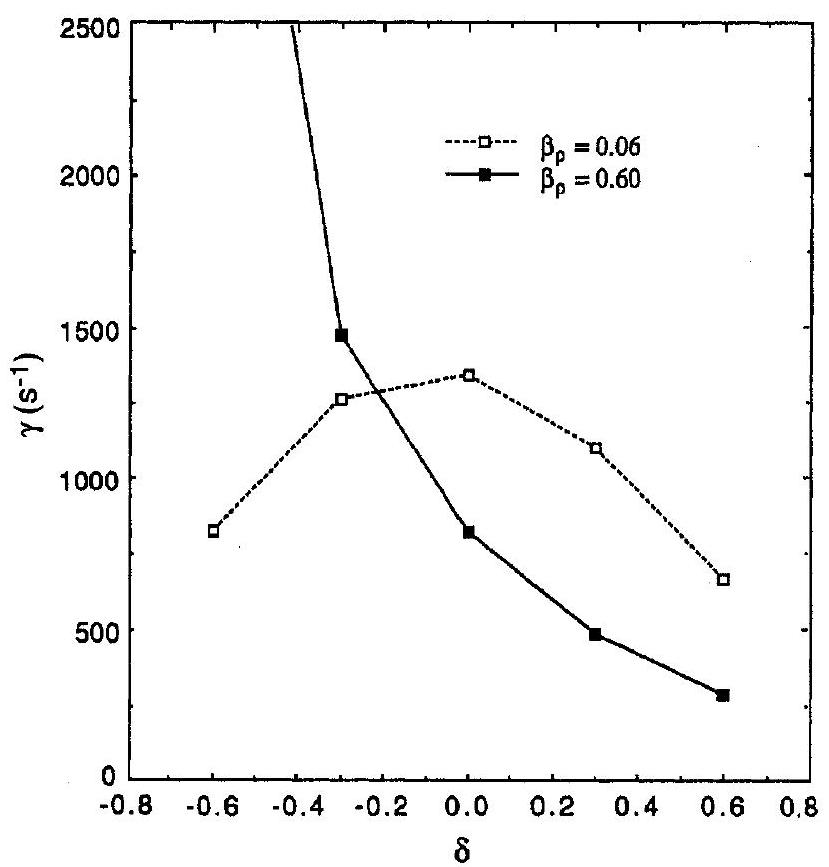
\includegraphics[max width=0.85\textwidth,max height=0.3\textheight]{2025_01_10_a0135324997886412d98g-6}
 \caption{\uline{Growth rates (in $\mathrm{s}^{-1}$ ) versus triangularity for a resistive wall conformal to the plasma shape at a midplane distance of $\mathrm{d}=1.3 \mathrm{a}$ for seversal shapes ranging from the inverse dee $(\delta=-0.6)$ to the regular dee $(\delta=0.6)$ at high beta $\left(\beta_{p}=0.6\right)$ and low beta $\left(\beta_{p}=0.06\right)$.\\}\\在高贝塔系数$\left(\beta_{p}=0.6\right)$ 和低贝塔系数$\left(\beta_{p}=0.06\right)$条件下,从反向笛形$(\delta=-0.6)$ 到正笛形$(\delta=0.6)$ ,与等离子体形状一致的电阻壁在中面距离$\mathrm{d}=1.3 \mathrm{a}$ 处的增长率(单位为$\mathrm{s}^{-1}$ )与三角形变的关系。}
  	\label{fig4.}
  \end{figure}
  
   \begin{figure}[H]
  	\centering
  	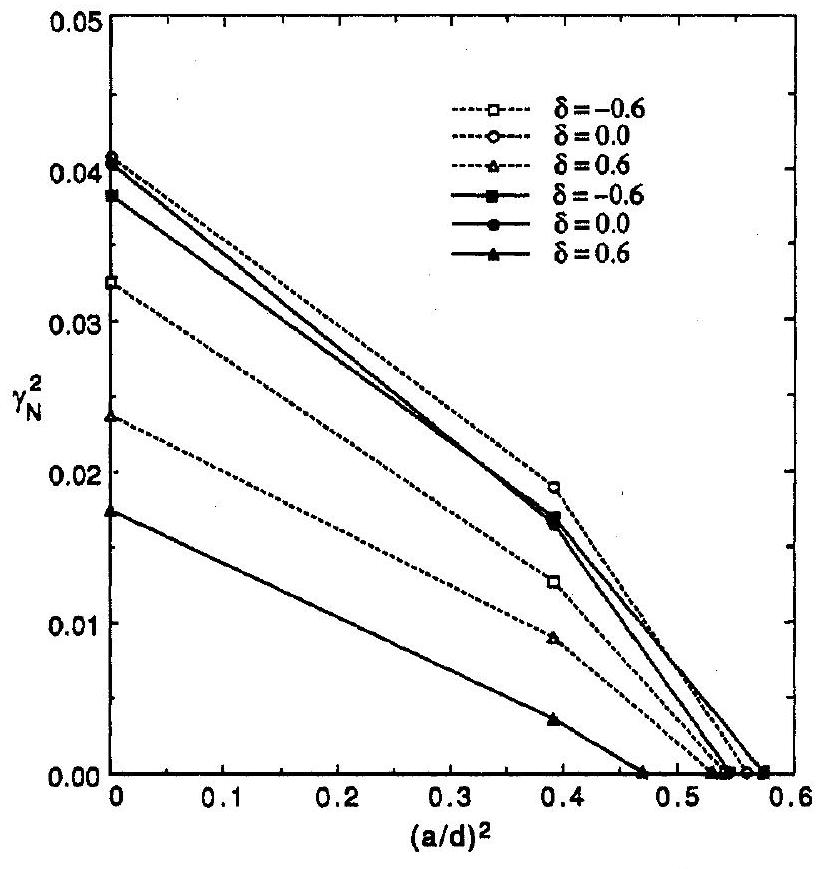
\includegraphics[max width=0.85\textwidth,max height=0.3\textheight]{2025_01_10_a0135324997886412d98g-6(1)}
 \caption{\uline{Plot of the square of the normalized ideal wall MHD growth rate $\gamma_{N}^{2}$ versus $\mathrm{a}^{2} / \mathrm{d}^{2}$, with an ideally conducting wall. The results are shown for three shapes (inverse dee, ellipse, regular dee) at high $\beta_{p}$ (solid symbols) and low $\beta_{p}$ (open symbols).}\\理想导电壁面的归一化理想壁面 MHD 增速 $\gamma_{N}^{2}$  与 $\mathrm{a}^{2} / \mathrm{d}^{2}$ 的平方关系图。图中显示了高$\beta_{p}$ (实心符号)和低$\beta_{p}$ (空心符号)时三种形状(反向笛形、椭圆形、规则笛形)的结果。}
  	\label{fig}
  \end{figure}
 
  
 \section{压力效应}
 {  \small PRESSURE EFFECTS \par }
  
 
\enzhbox{  The operational diagrams in Figs 1 and 3 show a much stronger stabilizing effect of $\epsilon \beta_{\mathrm{p}}$ in the DIII-Dlike cross-section ( $\kappa=2.5, \delta=0.6, \lambda=0$ ) than for the TCV dee shape ( $\kappa=3.0, \delta=0.5, \lambda=0.2$ ).}{
\textcolor{blue}{图 1} 和\textcolor{blue}{图 3} 中的运行图显示,$\epsilon \beta_{\mathrm{p}}$  在 DIII-D 样横截面($\kappa=2.5, \delta=0.6, \lambda=0$  )上的稳定作用比 TCV dee 形($\kappa=3.0, \delta=0.5, \lambda=0.2$  )要大得多。}
  
 
\enzhbox{  Figure 3 shows that the most important reason for this difference is the more triangular shape of DIII-D (note that a positive $\lambda$ decreases the effective triangularity \textcolor{green!50!black}{[9]}). The strong dependence of the pressure effect on triangularity is illustrated by Fig. 4. This figure shows resistive wall growth rates for elongated crosssections ( $\kappa=2.5, A=3$ ) at low and high pressures ( $\beta_{p}=0.06$ and 0.6 , respectively) and at several different triangularities ranging from $\delta=-0.6$ (inverse dee) to $\delta=+0.6$ (standard dee). The wall is a conformal copy of the plasma surface with minor radius $d=1.3 a$ and has the same resistivity and thickness as the TCV vacuum vessel used for Fig. 1. Pressure is strongly destabilizing for the inverse dee, somewhat stabilizing for the ellipse and clearly stabilizing for the standard dee. The inverse dee is strongly destabilized, and with $\beta_{\mathrm{p}}=0.6$ the mode is near marginal stability with an ideally conducting wall, see Fig. 5.}{
\textcolor{blue}{图 3} 显示,造成这种差异的最重要原因是 DIII-D 的三角形变多(注意正 $\lambda$  会降低有效三角形变 \textcolor{green!50!black}{[9]})。\textcolor{blue}{图 4} 说明了压力效应对三角形变的强烈依赖性。该图显示了拉长截面($\kappa=2.5, A=3$  )在低压和高压(分别为$\beta_{p}=0.06$  和 0.6)以及从$\delta=-0.6$  (逆三角形变)到$\delta=+0.6$  (标准三角形变)的几种不同三角形下的阻力壁生长率。腔壁是等离子体表面的共形副本,小半径为 $d=1.3 a$ ,电阻率和厚度与\textcolor{blue}{图 1} 中使用的 TCV 真空腔体相同。压力对反笛声具有强烈的失稳作用,对椭圆形具有一定的稳定作用,对标准笛声具有明显的稳定作用。反笛声具有强烈的失稳性,在理想的导电壁上,$\beta_{\mathrm{p}}=0.6$  模式接近临界稳定,见\textcolor{blue}{图 5}。}
  
 
\enzhbox{  Figure 5 shows the square of the normalized ideal wall MHD growth rate (a measure of the ideal MHD driving energy) versus the reciprocal wall radius squared for three different triangularities ( $\delta=-0.6$, $0.0,0.6$ ) and for both high and low pressures. The dee shape is clearly the most stable among all the cases. For this configuration, a finite pressure is significantly stabilizing in the absence of a wall and remains so when wall stabilization is accounted for.}{
\textcolor{blue}{图 5} 显示了三种不同三角形变($\delta=-0.6$ 、$0.0,0.6$  )以及高压和低压下归一化理想壁 MHD 增长率(理想 MHD 驱动能的量度)与倒数壁半径平方的关系。在所有情况下,dee 形显然是最稳定的。对于这种位形,在没有壁的情况下,有限压力具有明显的稳定作用,当考虑到壁的稳定作用时,情况依然如此。}
  
 
\enzhbox{  By contrast, for the inverse dee, pressure is clearly destabilizing both with and without a wall. The critical wall distance for the inverse dee is quite close to $d=1.3 a$, and therefore the resistive wall growth rate (with the wall at that position) is very large in Fig. 4 for that case. For the pure ellipse, the free space growth rate is virtually the same for the low and high pressure cases, but high pressure shows a stabilizing influence in the presence of a wall, and the growth rate falls below that for the inverse dee as the wall is moved inward.}{
相比之下,对于逆笛声,无论有壁还是无壁,压力都会明显失稳。反氐的临界壁距非常接近 $d=1.3 a$ ,因此在\textcolor{blue}{图 4} 中,该情况下的阻力壁增长率(壁在该位置时)非常大。对于纯椭圆,低压和高压情况下的自由空间增长率几乎相同,但高压在有壁的情况下显示出稳定的影响,当壁向内移动时,增长率低于逆笛声的增长率。}
  
 
\enzhbox{  Plots of the equilibrium flux surfaces show that, for the dee shape, increased pressure reduces the central elongation. This can be interpreted as the result of squeezing in the vertical direction by the combination of triangular shape and the Shafranov shift. The same effect leads to an increased elongation at high $\beta_{p}$ in an inverse dee.}{
平衡磁面图显示,对于 dee 形,压力增加会降低中心伸长率。这可以解释为三角形变和 Shafranov 位移相结合在垂直方向上产生挤压的结果。同样的效应导致反向氐型在高$\beta_{p}$ 处的伸长率增大。}
  
 
 
\enzhbox{  We conclude that the primary effect of pressure on the dee shape is to lower the free space driving energy. Conversely, pressure increases the free space energy for the inverse dee. Thus, the favourable effect of pressure shown in the operational diagrams, Figs 1 and 3 , is mainly due to the lowering of the free space driving energy and not to its effect on the wall coupling. For the ellipse, the free space growth rates are virtually unaffected by pressure, but there is an increase in the wall stabilization for the high pressure case.}{
我们得出结论,压力对 dee 形状的主要影响是降低自由空间驱动能。相反,压力会增加反向 dee 的自由能。因此,运行图(\textcolor{blue}{图 1} 和\textcolor{blue}{图 3})中显示的压力的有利影响主要是由于降低了自由空间驱动能,而不是其对壁面耦合的影响。对于椭圆,自由空间增长率几乎不受压力的影响,但在高压情况下,壁面稳定性会增加。}
  
 \section{电流剖面效果}
 {  \small CURRENT PROFILE EFFECTS \par }
 
\enzhbox{  It is well known that the current profile strongly influences the vertical stability. The almost identical results for different classes of current profiles in Fig. 1 show that the relevant parameter characterizing the current distribution is the internal inductance. Flat current profiles with low internal inductance lead to stronger coupling between the plasma and the external conductors. However, we find computationally that, in the absence of a conducting shell, the growth rate generally increases with decreasing inductance (see also Ref. \textcolor{green!50!black}{[20]}). This is shown in Fig. 6, where the ideal wall growth rate is plotted as a function of the wall radius for two DIII-D shaped equilibria with different internal inductances, $l_{\mathrm{i}}=0.6$ and 0.8 , respectively.}{
众所周知,电流剖面对垂直稳定性有很大影响。\textcolor{blue}{图 1} 中不同类型电流剖面的结果几乎相同,这表明表征电流分布的相关参数是内电感。低内电感的扁平电流剖面会导致等离子体与外部导体之间更强的耦合。然而,我们在计算中发现,在没有导电外壳的情况下,增长率通常会随着电感的减小而增加(另见参考文献 \textcolor{green!50!black}{[20]})。如\textcolor{blue}{图 6} 所示,图中绘出了两个具有不同内部电感 $l_{\mathrm{i}}=0.6$  和 0.8 的 DIII-D 形平衡态的理想壁生长率与壁半径的函数关系。}
  
 
\enzhbox{  Peaking of the current profile is evidently stabilizing when the wall is distant but destabilizing when the wall is sufficiently close. At a wall distance of roughly $d=1.4 a$, the two curves in Fig. 6 cross, and the growth rate is independent of the inductance. This point is close to the critical wall distance. Therefore, the internal inductance has a rather small effect on the marginal position of the ideal wall, but it has a much stronger effect on the resistive growth rates with a close fitting wall \textcolor{green!50!black}{[14]}. In fact, with the wall at $d=1.3 a$, the two cases in Fig. 6 have nearly a factor of two difference in the resistive growth rate. The reduction of the free space growth rate with increasing inductance appears to be due mainly to a reduction of the ellipticity of the central flux surfaces. It should be noted that there are many competing effects, for example a similar reduction of the central triangularity, which reduces the finite pressure stabilization. In addition, peaking of the current profile effectively increases the aspect ratio, so that the toroidal stabilization is reduced. However, as discussed in Section 3, the toroidal stabilization is insignificant for highly elongated cross-sections.\\}{
显然,当壁距离较远时,峰化电流剖面会趋于稳定,但当壁距离足够近时,峰化电流剖面会失稳。在壁距约为 $d=1.4 a$ 时,\textcolor{blue}{图 6} 中的两条曲线交叉,增长率与电感无关。这一点接近临界壁距。因此,内部电感对理想壁面的临界位置影响相当小,但它对贴合壁面的电阻增长率的影响要大得多\textcolor{green!50!black}{[14]}。事实上,当壁位于 $d=1.3 a$ 时,\textcolor{blue}{图 6} 中两种情况的电阻增长率相差近 2 倍。自由空间增长率随电感量增加而降低,这似乎主要是由于中心磁面的椭圆度降低所致。需要注意的是,还有许多竞争效应,例如类似的中心三角形变的减小,会降低有限压力的稳定性。此外,峰化电流剖面会有效增加环径比,从而降低环径稳定度。然而,正如第 3 节所讨论的,环形稳定对于高度拉长的横截面来说并不重要。}
  \begin{figure}[H]
  	\centering
  	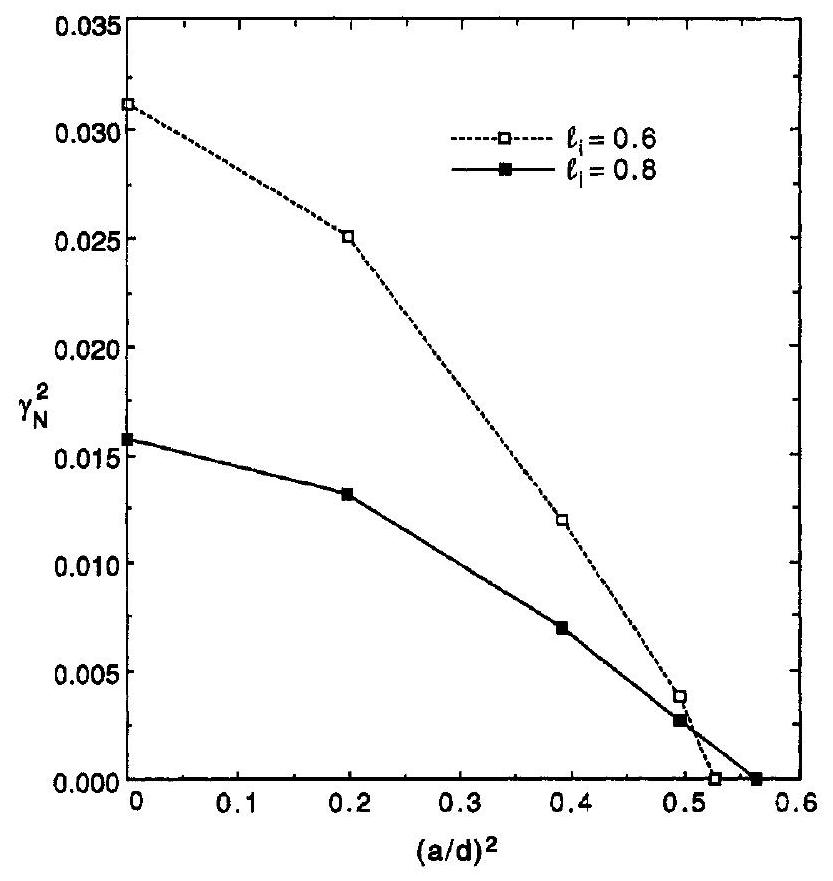
\includegraphics[max width=0.85\textwidth,max height=0.3\textheight]{2025_01_10_a0135324997886412d98g-7}
 \caption{\uline{Plot of $\gamma_{N}^{2}$ versus $\mathrm{a}^{2} / \mathrm{d}^{2}$ with an ideally conducting wall for DIII-D-like equilibria with no pressure for $1_{i}=0.6$ (dashed curve) and for $1_{i}=0.8$ (solid curve).}\\在 DIII-D 类无压力平衡条件下,$1_{i}=0.6$ (虚线)和$1_{i}=0.8$ (实线)的$\gamma_{N}^{2}$ 与$\mathrm{a}^{2} / \mathrm{d}^{2}$ 的关系曲线图。}
  	\label{fig6.}
  \end{figure}
  
   
 \subsection{通过分立导体实现被动稳定}
 {  \small Passive stabilization by discrete conductors \par }
 
\enzhbox{  While the effect of broadening the current profile increases the destabilizing force on the equilibrium, it also increases the stabilizing effect of a completely surrounding conducting wall. The balance between these competing effects is changed if the passive stabilization is provided primarily by discrete conductors instead of a complete, surrounding wall. As an example, we consider the configuration indicated in Fig. 7. The equilibrium has $\kappa=1.9, \delta=0.7$ and $A=4.54$. Figure 8 shows that in this configuration the growth rate increases with decreasing $l_{\mathrm{i}}$. This effect has been observed previously by Pearlstein \textcolor{green!50!black}{[23]} and by Jardin \textcolor{green!50!black}{[24]}.}{
虽然拓宽电流剖面的效果会增加对平衡的失稳力,但同时也会增加完全环绕的导电墙的稳定效果。如果被动稳定作用主要由离散导体而非完整的环绕壁提供,那么这些相互竞争的效应之间的平衡就会发生变化。例如,我们考虑\textcolor{blue}{图 7} 所示的位形。平衡点为 $\kappa=1.9, \delta=0.7$  和 $A=4.54$ 。\textcolor{blue}{图 8} 显示,在这种位形中,增长率随着 $l_{\mathrm{i}}$ 的减小而增加。Pearlstein \textcolor{green!50!black}{[23]} 和 Jardin \textcolor{green!50!black}{[24]} 以前也观察到过这种效应。}
  
 
\enzhbox{  An interesting comparison is obtained by replacing the discrete conductors by the complete wall, as indicated by a dotted contour in Fig. 7. The total wall resistance was normalized to that of the passive conductors. Figure 8 shows that with the closed wall configuration the growth rate decreases monotonically with decreasing $l_{\mathrm{i}}$.}{
如\textcolor{blue}{图 7} 中的虚线等值线所示,将分立导体替换为完整的墙体,可获得有趣的比较结果。壁的总电阻与无源导体的电阻进行了归一化处理。\textcolor{blue}{图 8} 显示,在封闭壁的位形下,增长率随着 $l_{\mathrm{i}}$ 的减小而单调降低。}
  
 
\enzhbox{  Figure 7 shows the contours of perturbed flux for the cases of (a) high and (b) low $l_{\mathrm{i}}$ in Fig. 8. While the coupling of the perturbed flux to the closed wall is improved in the low $l_{i}$ case, the coupling to the discrete conductors is not. Therefore, the increase in the destabilizing force due to the broader current profile dominates, and the growth rate increases with decreasing $l_{\mathrm{i}}$.}{
	\textcolor{blue}{图 7} 显示了\textcolor{blue}{图 8} 中(a)高$l_{\mathrm{i}}$ 和(b)低$l_{\mathrm{i}}$ 情况下的扰动通量等值线。在低$l_{i}$ 情况下,扰动通量与封闭壁的耦合得到改善,但与离散导体的耦合却没有改善。因此,更宽的电流剖面导致的失稳力的增加占主导地位,增长率随$l_{\mathrm{i}}$的减小而增加。}


  \begin{figure}[H]
  	\centering
  	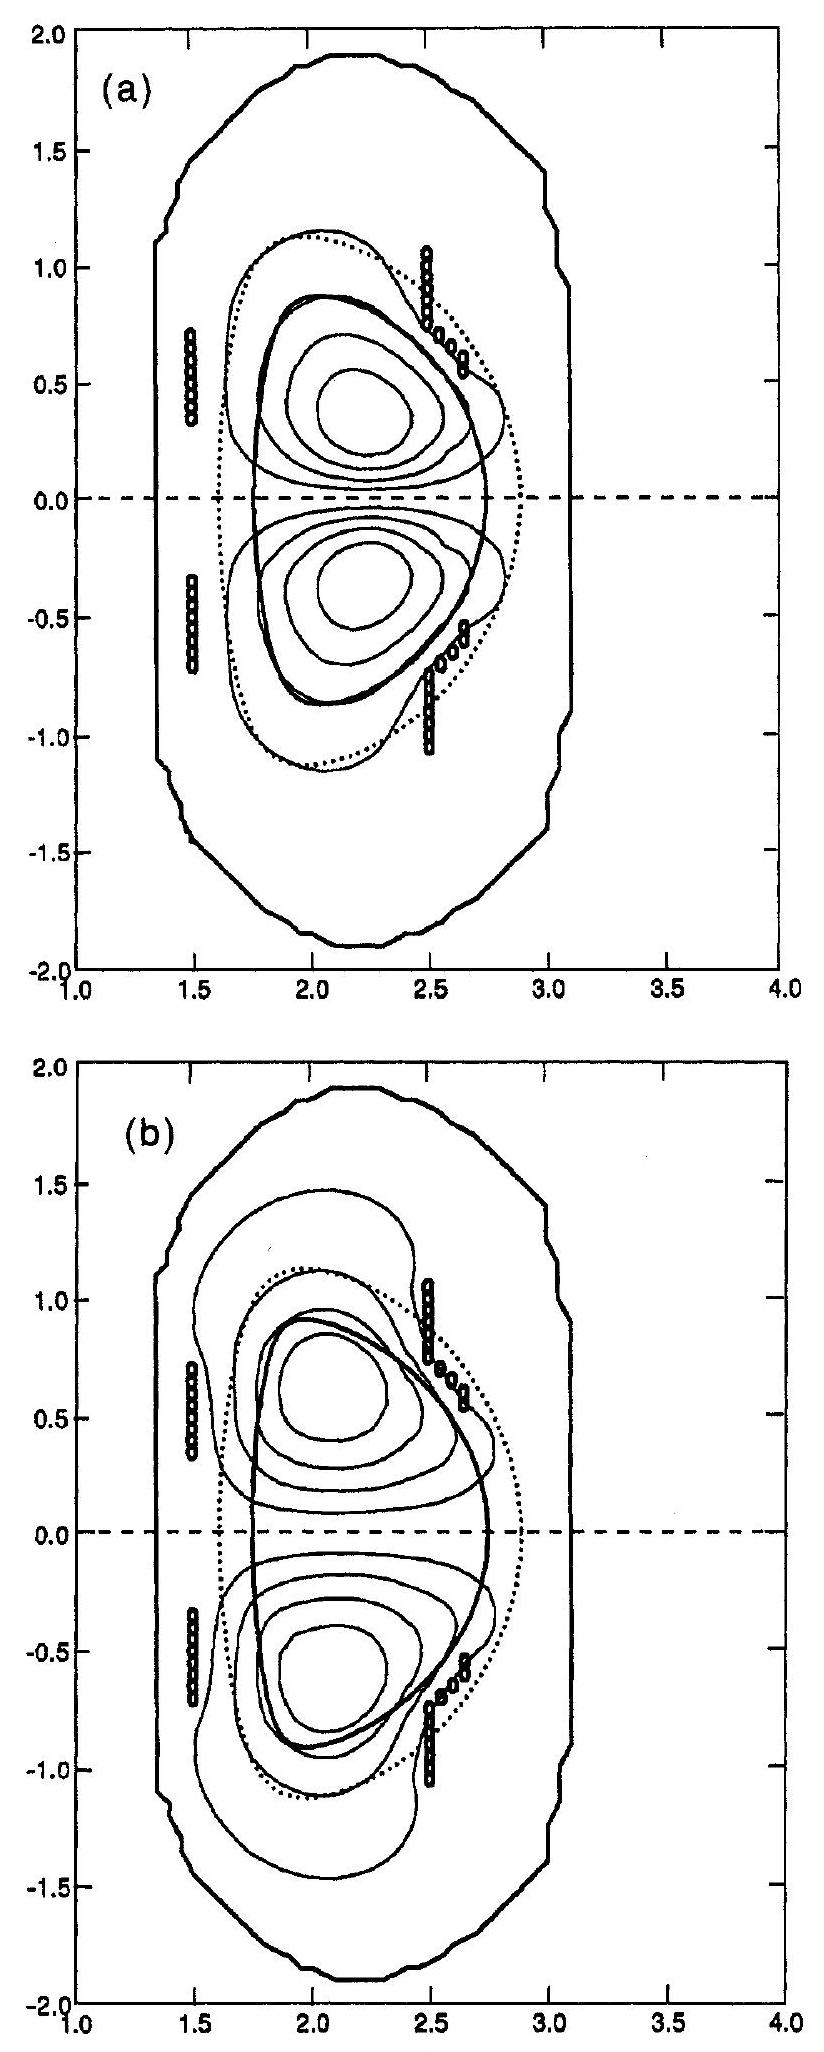
\includegraphics[max width=0.85\textwidth,max height=0.5\textheight]{2025_01_10_a0135324997886412d98g-8(1)}
 \caption{\uline{The plasma boundary, the discrete conductor sets and (shown as a dotted contour) a fictitious completely surrounding wall for the comparison in Fig. 8. The vacuum vessel is quite distant from the plasma. The perturbed flux contours are shown for two equilibria with (a) high $1_{i}$ and (b) low $1_{i}$ in the configuration with discrete conductors.\\}\\\textcolor{blue}{图 8} 中的等离子体边界、离散导体组和(以虚线等高线表示)虚构的完全环绕的壁,用于比较。真空腔体远离等离子体。扰动通量等值线显示了在有离散导体的位形中,(a) 高 $1_{i}$  和 (b) 低 $1_{i}$  两种平衡状态下的扰动通量等值线。}
  	\label{fig7.}
  \end{figure}
  
   \begin{figure}[H]
  	\centering
  	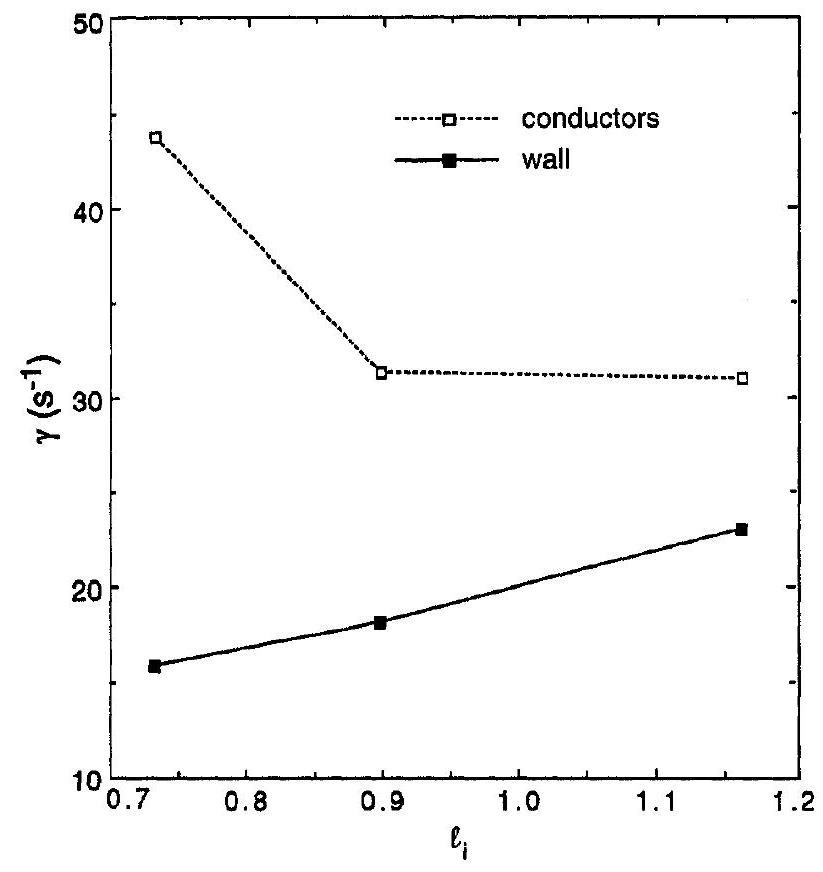
\includegraphics[max width=0.85\textwidth,max height=0.3\textheight]{2025_01_10_a0135324997886412d98g-8}
 \caption{\uline{Growth rates (in $s^{-1}$ ) versus $1_{i}$ for the configuration in Fig. 7 stabilized by discrete conductors with the vacuum vessel far from the plasma. For comparison, growth rates are shown with a completely surrounding wall (conformal to the plasma surface at $\mathrm{d}=1.3 \mathrm{a}$ ).\\}\\\textcolor{blue}{图 7} 中由离散导体稳定的真空腔体远离等离子体时的增长率(单位为 $s^{-1}$  )与 $1_{i}$  的关系。为便于比较,图中显示了完全环绕的壁(在 $\mathrm{d}=1.3 \mathrm{a}$  处与等离子体表面共形)的增长率。}
  	\label{fig8.}
  \end{figure}
  
 
 
 
\enzhbox{  We conclude that, for highly elongated tokamaks, there are two main effects of the internal inductance on vertical stability. Firstly, wall stabilization is improved for low internal inductance because of increased magnetic coupling. Secondly, current peaking reduces the shaping of the internal flux surfaces, which reduces the instability growth rate in the absence of a wall. For highly elongated, feedback stabilized discharges with a closed wall, the effect on wall coupling is more important, and stability improves at low inductance. However, when there is not a completely surrounding wall, the competition of these two effects is more subtle and depends on the details of the current profile and of the placement of the conductors.}{
我们的结论是,对于高度拉长的托卡马克,内部电感对垂直稳定性有两个主要影响。第一,由于磁耦合增加,低内电感会改善壁的稳定性。其次,电流峰值减少了内部磁面的塑形,从而降低了无壁情况下的不稳定性增长率。对于具有封闭壁的高拉长反馈稳定放电,对壁耦合的影响更为重要,在低电感时稳定性也会提高。然而,当没有完全环绕的壁时,这两种效应的竞争更为微妙,并取决于电流剖面和导体放置的细节。}
  
 \section{结 论}
 {  \small CONCLUSIONS \par }
 
\enzhbox{  We have found that high values of $\epsilon \beta_{\mathrm{p}}$ significantly improve the vertical stability of dee shaped tokamaks.}{
我们发现,$\epsilon \beta_{\mathrm{p}}$ 值越高,「笛形 」托卡马克的垂直稳定性就越好。}
  
 
\enzhbox{  The effect can be described in terms of an almost linear dependence of the critical internal inductance on $\epsilon \beta_{\mathrm{p}}, l_{\mathrm{i}, \text { crit }} \approx l_{\mathrm{i}, 0}+c \epsilon \beta_{\mathrm{p}}$. Comparison between different cross-sections shows that the coefficient $c$ increases strongly with triangularity and decreases somewhat with elongation. For a DIII-D-like cross-section, the dependence of $l_{\mathrm{i}, \text { crit }}$ on $\epsilon \beta_{\mathrm{p}}$ is quite pronounced. This effect is beneficial for reaching high beta, because it increases the maximum stable elongation or, alternatively, allows the current profile to be more peaked, which increases the beta limit due to the $n=1$ external kink mode $\textcolor{green!50!black}{[2,9]}$.}{
这种效应可以用临界内电感与 $\epsilon \beta_{\mathrm{p}}, l_{\mathrm{i}, \text { crit }} \approx l_{\mathrm{i}, 0}+c \epsilon \beta_{\mathrm{p}}$ 几乎呈线性关系来描述。不同横截面之间的比较表明,系数 $c$  随三角形变而强烈增加,随伸长而有所减小。对于类似 DIII-D 的横截面,$l_{\mathrm{i}, \text { crit }}$  与 $\epsilon \beta_{\mathrm{p}}$  的关系非常明显。这种效应有利于达到高贝塔值,因为它增加了最大稳定伸长率,或者说,使电流剖面更加峰化,从而增加了由于$n=1$ 外扭曲模$\textcolor{green!50!black}{[2,9]}$而导致的贝塔极限。}
  
 \section{致谢}
 {  \small ACKNOWLEDGEMENTS \par }
 
\enzhbox{  This work was supported in part by the Swiss National Science Foundation. We acknowledge the work of H . Lütjens in adapting the CHEASE equilibrium code for NOVA-W.}{
这项工作得到了瑞士国家科学基金会的部分支持。我们感谢 H .Lütjens 为 NOVA-W 修改 CHEASE 平衡代码所做的工作。}
  \setlength{\parskip}{0pt} \small % ==document body ends
 \section{REFERENCES}
\textcolor{green!50!black}{[1]} TROYON, F., et al., Plasma Phys. Control. Fusion 26 (1984) 209.\\[0pt]
\textcolor{green!50!black}{[2]} LAZARUS, E.A., et al., Phys. Fluids B 3 (1991) 2220; LAZARUS, E.A., et al., Phys. Fluids B 4 (1992) 3644.\\[0pt]
\textcolor{green!50!black}{[3]} YUSHMANOV, P.N., et al., Nucl. Fusion 30 (1990) 1999.\\[0pt]
\textcolor{green!50!black}{[4]} ZAKHAROV, L.E., Sov. Phys. - Tech. Phys. 16 (1971) 645 (English translation: Zh. Tekh. Fiz. 41 (1971) 823).\\[0pt]
\textcolor{green!50!black}{[5]} MUKHOVATOV, V.S., SHAFRANOV, V.D., Nucl. Fusion 11 (1971) 605.\\[0pt]
\textcolor{green!50!black}{[6]} LAZARUS, E.A., et al., Nucl. Fusion 30 (1990) 111.\\[0pt]
\textcolor{green!50!black}{[7]} HOFMANN, F., et al., in Fusion Technology 1986 (Proc. 14th Symp. Avignon, 1986), Vol. 1, Pergamon Press, Oxford (1986) 687.\\[0pt]
\textcolor{green!50!black}{[8]} TAYLOR, T.S., et al., in Plasma Physics and Controlled Nuclear Fusion Research 1990 (Proc. 13th Int. Conf. Washington, DC, 1990), Vol. 1, IAEA, Vienna (1991) 177 ; LAO, L.L., et al., Phys. Fluids B 4 (1992) 232.\\[0pt]
\textcolor{green!50!black}{[9]} ERIKSSON, G., et al., in Plasma Physics (Proc. 1992 Int. Conf. Innsbruck), Vol. 16C, Part I, European Physical Society (1992) 343.\\[0pt]
\textcolor{green!50!black}{[10]} ZARNSTORFF, M.C., et al., in Plasma Physics and Controlled Nuclear Fusion Research 1990 (Proc. 13th Int. Conf. Washington, DC, 1990), Vol. 1, IAEA, Vienna (1991) 109.\\[0pt]
\textcolor{green!50!black}{[11]} LÜTJENS, H., et al., Comput. Phys. Commun. 69 (1992) 287.\\[0pt]
\textcolor{green!50!black}{[12]} WARD, D.J., et al., J. Comput. Phys. 104 (1993) 221.\\[0pt]
\textcolor{green!50!black}{[13]} LAVAL, G., et al., Phys. Fluids 17 (1974) 835.\\[0pt]
\textcolor{green!50!black}{[14]} HANEY, S.W., FREIDBERG, J.P., Phys. Fluids B 1 (1989) 1637.\\[0pt]
\textcolor{green!50!black}{[15]} ERIKSSON, H.G., Plasma Phys. Control. Fusion 34 (1992) 1721.\\[0pt]
\textcolor{green!50!black}{[16]} REBHAN, E., Nucl. Fusion 15 (1975) 277.\\[0pt]
\textcolor{green!50!black}{[17]} REBHAN, E., SALAT, A., Nucl. Fusion 16 (1976) 805.\\[0pt]
\textcolor{green!50!black}{[18]} HOFMANN, F., SCHULTZ, C.G., in Controlled Fusion and Plasma Physics (Proc. 16th Eur. Conf. Venice, 1989), Vol. 13B, Part I, European Physical Society (1987) 335.\\[0pt]
\textcolor{green!50!black}{[19]} BERNARD, L.C., et al., Nucl. Fusion 18 (1978) 1331.\\[0pt]
\textcolor{green!50!black}{[20]} BECKER, G., LACKNER, K., in Plasma Physics and Controlled Nuclear Fusion Research 1976 (Proc. 6th Int. Conf. Berchtesgaden, 1976), Vol. 2, IAEA, Vienna (1977) 401.\\[0pt]
\textcolor{green!50!black}{[21]} STAMBAUGH, R.D., et al., Nucl. Fusion 32 (1992) 1642.\\[0pt]
\textcolor{green!50!black}{[22]} WARD, D.J., JARDIN, S.C., Nucl. Fusion 32 (1992) 973.\\[0pt]
\textcolor{green!50!black}{[23]} PEARLSTEIN, L.D., Lawrence Livermore National Laboratory, personal communication, 1992.\\[0pt]
\textcolor{green!50!black}{[24]} JARDIN, S.C., Plasma Physics Laboratory, Princeton University, personal communication, 1992.\\
(Manuscript received 21 December 1992\\
Final manuscript received 29 March 1993)

  
  	%----------------------------------------------------------------------------------------
  \end{sloppypar}	
  \begin{flushright}
  	\vfill \footnotesize
  	——本翻译PDF由Paper_translator生成, \url{https://github.com/DertahSama/Paper_translator}
  \end{flushright}
  \end{document}
